%%%%%%%%%%%%%%%%%%%%%%%%%%%%%%%%%%%%%%%%%%%%%%%%%%%%%%%%%%%%%
\chapter{Oil production methods}
%\addcontentsline{toc}{chapter}{Introduction}

\section*{Need for energy}

Modern industrial societies consume large quantities of energy in order to 
maintain todays high standard of living. Most of that energy comes as a 
result of the technology of oil production.  According to the U.S. Energy 
Information Administrations (EIA) International Energy Outlook 2016, the global 
supply of crude oil, other liquid hydrocarbons, and biofuels is expected to be 
adequate to meet the world's demand for liquid fuels through 2040. There is 
substantial uncertainty about the levels of future liquid fuels supply and 
demand. According to current prognosis, oil production in matured reservoirs is 
expected to decline and this could create gap between supply and demand of 
hydrocarbons in various parts of the world. To counterpart
this growing demand-supply discrepancy,the petroleum industry will have to give more
attention to their mature fields to sustain current production levels. It should be
realized that most operators have not exploited the full capacity of mature fields
to their potential. In addition to this they face the challenge of developing green
fields in such a way that they can be produced to their maximum potential in
the future. With a mean recovery factor of about 36\%, there is an immense
opportunity for ``production optimization''.

The primary objective within reservoir management is to provide optimal
production scenarios, accompanied by estimates of expected hydrocarbon recovery,
ultimately resulting in an optimized field development plan. Elements of such a plan
include recovery techniques, well types and position or pattern designs, completion
types, and production scheduling. In fields with significant complexity, automated
workflows based on numerical algorithms will need to be used to find optimal
choices for all these variables.



\section{Oil production methods} \label{sec:OilProductionMethods}

During the life of a producing oil field, several production stages are 
encountered. Initially, when a field is brought into production, oil flows 
naturally to the surface due to current reservoir pressure in the primary stage. 
As reservoir pressure drops, water is typically injected to boost the pressure, 
so that it displaces the oil in the so called ``secondary'' stage. Lastly, the 
remaining oil can be recovered by a variety of methods such as \ce{CO2} injection, natural gas 
miscible injection, and steam recovery in a tertiary or enhanced oil recovery (EOR) 
phase 
\citep{Meyer}. 

\section{Primary recovery}
Glover \citep{Glover} explained all recovery methods, 
including primary recovery mechanism as it is the stage when the natural energy 
of the reservoir is used to transport hydrocarbons towards and out of the 
production wells. The earliest possible determination of the drive mechanism is 
a primary goal in the early life of the reservoir, as its knowledge can greatly 
improve the management and recovery of reserves from the reservoir in its middle 
and later life. There are five important drive mechanisms: (i) Solution gas 
drive; (ii) Gas cap drive; (iii) Water drive; (iv) Gravity drainage; (v) 
Combination or mixed drive. All these mechanisms maintain the reservoir pressure, 
though water drive maintains much higher pressure than the gas drive mechanisms (Figure 1.2).
\begin{description}[style=nextline]
\item [\textbf{Solution gas drive}] 
In solution gas drive, the expansion of the dissolved gases 
in the oil and water provides most of the reservoirs drive energy.
Oil recovery from this type is typically between 20\% and 30\% of original oil in place.
% Solution Gas Drive is associated to two types of Reservoirs that are related to pressure; 
%under saturated reservoirs (no free gases in oil), drive energy is provided only 
%by the bulk expansion of the reservoir rock and liquids; saturated reservoirs, 
%where the pressure is less than the bubble point pressure. A decline in 
%reservoir pressure causes bubbles of gas to expand. Thus gas expansion is the 
%primary reservoir drive for reservoirs below the bubble point. 

\begin{figure}[ht]
\begin{center}
      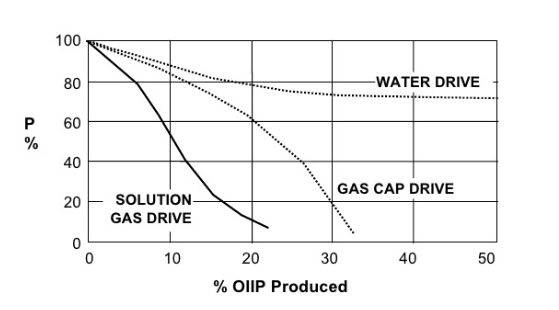
\includegraphics[width=8cm, height=5cm]{figures/ReservoirPerformancePrimary.png}
       \end{center}
     \caption{Pressure trends under various drive mechanisms.}
  \label{fig:ReservoirPerformancePrimary}
\end{figure}

\item[\textbf{Gas cap drive}] 
As production continues, the gas cap expands pushing the gas-oil 
contact (GOC) downwards. Eventually the GOC will reach the production wells and 
the gas oil ratio (GOR) will increase by large amounts. The recovery of gas cap 
reservoirs can be (20\% to 40\% OOIP). 
%Produced gas can be separated and immediately injected back into gas cap.
\item[\textbf{Water drive}]
The drive energy is provided by an aquifer that interfaces with the oil in the reservoir at the 
oil-water contact (OWC). The recovery from water driven reservoirs is usually good (20-60\% OOIP). 
%As production continues, and oil is extracted from the reservoir, the aquifer expands into the reservoir displacing the oil. 
%Oil production from a strongly water driven reservoir remains fairly constant until 
%water breakthrough occurs. When water breakthrough does occur the well can 
%either be shut-down, or assisted using gas lift.
\item[\textbf{Gravity drainage}]
Gravity drainage is the fourth drive force that might be 
considered for drive mechanism where the density differences between oil and gas 
and water result in their natural segregation in the reservoir. This process is relatively weak and in practice is only 
used in combination with other drive mechanisms. 
%\subsection*{Combination drive}
%In practice a reservoir usually incorporates at least two 
%main drive mechanisms. Therefore, Combination or Mixed Drive can be accounted as 
%the fifth type of Drives \citep{Glover}. Oil lifting by gas or pumps: In 
%addition to the previous drive mechanisms, artificial lifting is considered as a 
%primary recovery, which is a process used to increase pressure within the 
%reservoir, when the natural drive energy of the reservoir is not strong enough 
%to push the oil to the surface. The two main categories of artificial lift 
%include pumping systems and gas lift. Gas lift method injects compressed gas 
%into the well to re-establish pressure, making it produce. On the other hand, 
%jack pumps are submersed and used to lift the oil to the surface \citep{Fleshman}.
\end{description}
\section{Secondary recovery}
After initial discover and production, typical oil reservoirs lose the drive 
mechanism of gas or water that originally forced the oil to the surface. The 
second stage of hydrocarbon production in which an external fluid such as water: 
usually named water flooding or water injection or gas: referred to as gas 
flooding or gas injection, is injected into the reservoir through injection 
wells. By secondary recovery methods, another 15-20\% may be produced.
\citep{Fleshman}.
\begin{description}[style=nextline]
\item[\textbf{Water flooding}]
Water Flooding is implemented by injecting water into a set of 
wells while producing from the surrounding wells. Water flooding projects are 
generally implemented to accomplish reservoir pressure maintenance and as a water drive to 
displace oil from the injector wells to the producer wells\citep{Fleshman}.
\item[\textbf{Gas flooding}]
This method is similar to water flooding in principal, and is used 
to maintain gas cap pressure even if oil displacement is not required. Usually 
the produced natural gas is re-injected to the reservoir in order to maintain 
reservoir pressure rather than to displace the hydrocarbon. 
\begin{figure}[ht]
\begin{center}
      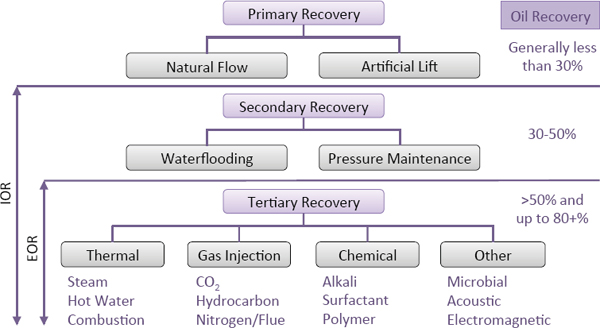
\includegraphics[width=10cm, height=6.5cm]{figures/OilRecoveryStages.png}
       \end{center}
     \caption{The different oil recovery stages and the corresponding oil recovery
factor.}
  \label{fig:OilRecoveryStages}
\end{figure}
%Traditional primary and secondary production methods typically recover one third 
%of oil in place, leaving two thirds behind. The reasons for this are not 
%difficult to understand. During the life of a well, there is always a point at 
%which the cost of producing an additional barrel of oil is higher than the price 
%the market will pay for that barrel. Production then halts. Under normal 
%circumstances, the well is abandoned, with 70\% of the oil left in the ground.
%Enhanced recovery techniques, EOR, can be used to recover additional 
%hydrocarbons. EOR introduces fluids that reduce viscosity and improve flow. 
%These fluids could consist of gases that are miscible with oil such as carbon 
%dioxide or nitrogen, steam, air or oxygen, polymer solutions, gels, 
%surfactant-polymer formulations, alkaline-surfactant-polymerformulations, or 
%microorganism formulations . However, the diagram of the oil recovery stages is 
%shown in Fig. 2 \citep{Lake_book89}.
\end{description}

\section{Enhanced oil recovery}
Enhanced oil recovery techniques refer to the recovery of oil through the injection of fluids and energy not 
normally present in the reservoir \citep{Romero}. The objectives of the 
injected fluids are to achieve mainly two purposes; First is to boost the 
natural energy in the reservoir; second is to interact with the reservoir 
rock/oil system to create conditions favourable for residual oil recovery that 
leads to reduce the interfacial tension between the displacing fluid and oil, 
increase the capillary number, reduce capillary forces, increase the drive water 
viscosity, provide mobility-control, create oil swelling, reduce oil viscosity, 
alter the wettability of reservoir rock \citep{Romero}. Enhanced oil 
recovery can be divided into two: thermal and non-thermal recovery \citep{Anazi}. Fig. 2 illustrates oil recovery stages by the different EOR 
techniques.
\subsection{Thermal techniques}
Thermal methods raise the temperature of the reservoir to heat the crude oil in 
the formation and therefore reduce its viscosity and/or vaporise part of the oil 
and thereby decrease the mobility ratio. The increase in heat reduces the 
surface tension, increases the permeability of the oil and improves the 
reservoir seepage conditions. The heated oil may also vaporise and then condense 
to be produced. This operation, however, requires substantial investment in 
special equipment. 
\begin{description}[style=nextline]
\item[\textbf{In-situ combustion (ISC)}]
In-situ combustion or fire flooding is a process in 
which an oxygen containing gas is injected into a reservoir where it reacts with 
the oil contained within the pore space to create a high temperature 
self-sustaining combustion front that is propagated through the reservoir. 
%The heat from the combustion thins out the oil around it, causes gas to vaporize 
%from it, and vaporizes the water in the reservoir to steam. Steam, hot water, 
%and gas, all act to drive oil in front of the fire to production wells. In-situ 
%combustion is possible if the crude-oil/rock combination produces enough fuel to 
%sustain the combustion front \citep{Romero}. Severe corrosion and 
%increased sand oil production are some of the problems that encountered by 
%implementation of this technique \citep{Romero}. 
\item[\textbf{Steam Injection}] 
Steam is injected into the reservoir either continuously or in 
cycles. %Continuous steam injection involves both injection and production wells, 
%whereas cyclic injection involves one well only which serves as both injection 
%and production well.
Steam floods are easier to control than in-situ combustion. 
For the same pattern size, the response time is 25-50\% lower than the response 
time for additional production by in-situ combustion \citep{Jelmert}.
\item[\textbf{Hot water flooding}]
Water-flooding in heavy oils is generally not an efficient 
way of production due to high viscosity of heavy oil compared to water. In hot 
water-flooding, thermal energy will increase oil mobility, and possibly improve
sweep efficiency \citep{Kermen}. 
%Injecting, regularly hot fresh to saline brines will improve oil recovery by dropping viscosity and decreasing 
%residual oil saturation. If low salinity waters are injected, clay matrix may 
%swell and therefore clog pore throats. Porosity and permeability can be 
%increased by collapsing some of the interlayer clays, when injecting water with 
%high temperature. According to \citep{Seni}, Burger and 
%others (1985) emphasized that although the incremental gain in production from 
%injecting hot water is substantial compared with that gained from injecting cold 
%water during typical water flood are less significant than those resulting from 
%injecting steam. Operators seldom employ hot water flooding because heat losses 
%in surface lines, wellbore, and formation are greater than the heat losses in 
%the other thermal processes. The heat losses reduce the processes effectiveness 
%in decreasing oil viscosity \citep{Ela}.
\end{description}
\subsection{Non thermal techniques}
\begin{description}[style=nextline]
\item[\textbf{Chemical Flooding}]
These processes use chemicals added to water in the injected fluid of a water 
flood to alter the flood efficiency in such a way as to improve oil recovery by: 
(i) Increasing water viscosity (polymer floods) (ii) Decreasing the relative 
permeability to water (cross-linked polymer floods) (iii) Increasing the 
relative permeability to oil (micellar and alkaline floods)  \citep{Glover} 
\item[\textbf{Polymer flooding}]
Polymers improve both vertical and areal sweep efficiency by 
reducing water-oil ratio. Polymers are injected through water injection wells in 
order to displace the residual oil. Increasing the displacing fluids viscosity 
and lowering its relative permeability through plugging \citep{Anazi}. 
\item[\textbf{Micelalr polymer flooding}]
It is well known that water and oil cannot be mixed 
until the third component, surfactant or soap, is added to reduce the 
interfacial tension between oil and water. Since micellar solution makes fluids 
miscible in the reservoir, almost 100\% of oil can be displaced especially in the 
presence of alkaline. However, due to reservoir rock non-uniformity in the field, the amount of oil recovered is reduced. 
 %The main objective of micellar injection is to reduce interfacial tension to enhance oil 
%recovery \citep{Zare}. 
%Micellar solutions are mixtures of surfactants, 
%co-surfactants, electrolytes, hydrocarbon, and water. Surfactants are substances 
%known as surface active agents, such as soap. Co-surfactants are used for 
%stability such as alcohols. Electrolytes are salts used to control viscosity and 
%interfacial tension such as sodium chloride or ammonium sulphate. \citep{Anazi}.
\item[\textbf{Alkaline-surfactant-polymer (ASP) flooding}]
During waterflooding residual oil is 
trapped due to low water viscosity and high water-oil interfacial tension, 
therefore another way is to inject the three chemicals; alkaline to minimize 
surface adsorption; surfactant to lower interfacial tension and stabilizes the 
emulsion. On the other hand, polymer is used to increase viscosity and to 
improve mobility control and sweep efficiency\citep{Kirk}. 
\end{description}
\subsection{ Nitrogen Injection}
%The nitrogen injection can be used in deep light to medium oil reservoirs mainly 
%containing \ce{C1} to \ce{C7} components. It is applicable in both the Sandstone and 
%Carbonate reservoirs.
Nitrogen itself is an inert gas that gets miscible at very 
high pressure and efficiently reduces the oil viscosity while providing efficient 
miscible displacement \citep{Syed}. Nitrogen can be used for the following
enhanced oil recovery applications: 
\begin{description}[style=nextline]
 \item [\textbf{Nitrogen immiscible flooding}]
%Gas cap displacement:The reservoir is a large anticlinal structure with a 
%sizable gas cap. 
Gas is being injected into the crest of the structure to 
maintain the pressure, to recover the hydrocarbon liquids in the gas cap, and to 
stabilize the gas/oil contact.
\item[\textbf{Nitrogen miscibility displacement mechanism}]
There are three types of miscibility including; First contact miscibility; Multi- contact miscibility; 
Vaporizing mass-transfer miscibility \citep{Shine}. 
\item[\textbf{Multi-contact miscibility}]
%In miscible flood processes some combination of transfer of components from the oil
%displaced to the injected fluid and from the injected fluid to the oil takes place as the phases flow through the porous 
%medium. Some hydrocarbon gases, with a high proportion of intermediate molecular 
%weight components (\ce{C3}, \ce{C4}, and\ce{C5}) are miscible with oil under pressure and 
%temperature conditions encountered in some oil reservoirs. Moreover, under much 
%wider condition the displacement of oil by hydrocarbon gases may lead, through 
%component exchange between oil and the gas, to creation of transition zone in 
%which the composition varies continuously between the composition of the 
%displacing fluid and the composition of the oil. Light to intermediate 
%components are exchanged between oil and injected fluid. A transition zone 
%spreads out in which both fluids are miscible. 
This type of miscibility is  subdivided into vaporizing gas drive, 
condensing gas drive\citep{Juttner}.

%\subsubsection*{Vaporising gas drive}
%It is a particular case of multiple contact 
%miscibility, based on the vaporization of intermediate components from the 
%reservoir oil to the injected gas creating a miscible transition zone. The \ce{\ce{C2}}-\ce{C5} 
%fraction is preferently extracted. This mainly occurs at high pressure, by 
%injecting natural (hydrocarbon) gas, flue gas or nitrogen. When Nitrogen is 
%injected at high pressure, it can form a miscible slug which aids in freeing the 
%oil from the reservoir rock.
%\subsubsection*{Gravity drainage}
%Gravity enhancement is by using the gravity drainage potential 
%of a dipping or thick hydrocarbon zone. (Nitrogen, which usually has a lower 
%density than the reservoir fluids, when injected into the crest or allowed to 
%migrate to the crest, will enhance the down dip displacement and production of 
%the reservoir fluids or of a gravity stable miscible slug) \citep{Clancy}.
%One of the most common gravity drainage processes is the Double 
%Displacement Process (DDP). This is done by injecting gas up -dip and producing 
%oil down-dip \citep{Shine}. By using Gravity Drainage, piston like 
%displacement is obtained, therefore gas fingering is avoided. In addition, the 
%following results are obtained: Horizontal gas-oil contact; gravity dominate the 
%gas flow; optimized time between gas injection and oil production as fast as 
%possible; the greater the dip angle the higher the injection and production 
%rates w/o gas fingering; the greater the dip the more effective the gravity 
%drainage \citep{Walker}.
\item[\textbf{Gas Flooding Injection}]
Gas is generally injected single or intermittently with water and this manner of 
injection called Water-Alternating-Gas (WAG), has become widely practiced over 
all of worlds oil fields \citep{Kulkarni}. According to miscibility 
between gas injected and oil displaced, gas injection can be classified into two 
major types: miscible gas injection and immiscible gas injection.
In miscible gas injection, the gas is injected at or above minimum miscibility 
pressure (MMP) which causes the gas to be miscible in the oil.
In contrast in immiscible gas injection, flooding by the gas is conducted below MMP. This low 
pressure injection of gas is used to maintain reservoir pressure to prevent 
production cut-off and thereby increase the rate of production \citep{Anazi}. 
In miscible flooding, the incremental oil recovery is obtained by one 
of the three mechanisms: oil displacement by solvent through the generation of 
miscibility (i.e. zero interfacial tension between oil and solvent hence 
infinite capillary number), oil swelling, and reduction in oil viscosity 
\citep{Kulkarni}. Miscible fluids are 100\% soluble in each other. The 
interfacial tension between miscible fluids is zero. Injection gases include:
\item[\textbf{LPG injection}]
Miscible LPG products such as ethane, propane, or butane have 
first contact miscibility, which means they will be miscible from the first 
contact with oil. However, LPGs are in such demand as marketable commodity that 
their use in EOR is limited \citep{Romero}. In particular, this process 
uses a slug of propane or other liquified petroleum gas (2 to 5\% of pore volume 
PV) followed by natural gas, inert gas, and/or water. Thus, the solvent will 
bank oil and water ahead, and fully displace all contacted oil \citep{Anazi}.
\item[\textbf{Enriched gas miscible process}]
In this process, a slug of methane (\ce{C1}) enriched 
with ethane (\ce{C2}), propane (\ce{C3}), or butane (\ce{C4}) (10\% to 20\% of the PV) and 
followed by lean gas and/or water is injected from water injection well into the 
reservoir. When the injected gas contacts virgin reservoir oil, \ce{C1}-\ce{C3} are 
quenched from the injected gas and absorbed into the oil \citep{Anazi}. 
The injected HC solvent is usually displaced with cheaper chase leaner or inert 
gas like Methane or Nitrogen. At reservoir conditions the most usual problem 
occurs with the hydrocarbon miscible flood is the gravity over-ride because of 
its lighter density than the oil and water. So that in any miscible flood the 
Minimum Miscibility Pressure (MMP) plays the most major role to overcome this 
problem. As a remedial factor the solvent is to be injected at or above the MMP 
of the reservoir fluid. Once it becomes miscible then it improves the sweep 
efficiency and fallouts in optimum recovery \citep{Syed}.
\item[\textbf{Carbon dioxide (\ce{CO2} ) injection}]
Is one of the most proven of these methods. Almost pure \ce{CO2} 
(>95\% of the overall composition) has the property of mixing with the oil to 
swell it, make it lighter, detach it from the rock surfaces, and causing the oil 
to flow more freely within the reservoir so that it can be swept up in the 
flow from injector well to producer well \citep{Melzer}. Flooding a 
reservoir with \ce{CO2} can occur either miscibility or immiscibly. Miscible \ce{CO2} 
displacement is only achieved under a specific combination of conditions, which 
are set by four variables: reservoir temperature, reservoir pressure, injected 
gas composition, and oil chemical composition. From a fundamental point of view, 
\ce{CO2} EOR works on a very simple principle, namely, that given the right physical 
conditions, \ce{CO2} will mix miscibly with oil, acting much like a thinning agent, 
the same way that gasoline does with motor oil. After miscible mixing, the fluid 
is displaced by a chase phase, typically water \citep{Meyer}. 
In this thesis \ce{CO2} injection as EOR method is going to by examined.
\end{description}
\section {Need for simulation and optimization}
Use of reservoir simulation has grown because of its ability to predict the 
future performance of oil and gas reservoirs over a wide range of operating 
conditions. Reservoir simulators use numerical methods and high-speed computers 
to model multidimensional fluid flow in reservoir rock. Technology improvements have enabled 
a widespread use of integrated simulation models for a better asset management 
to be fully combined with measured field data. Reliable simulators and 
adequate computing capacity are available to most reservoir engineers, so 
simulation is usually practical for all reservoir sizes and all types of 
reservoir performance studies. Although the use of simulation frequently is 
optional, it may be the only reliable way to predict the performance of a large, 
complex reservoir, especially if such external considerations as government 
regulations influence the production schedule. Even for small reservoirs where 
simple calculations or extrapolations may be adequate, simulation is often 
faster, cheaper, and more reliable than alternative methods for predicting 
performance.\citep{Mattax}

In petroleum fields, hydrocarbon production is often constrained by reservoir 
conditions, deliverability of the pipeline network, fluid handling capacity of 
surface facilities, safety and economic considerations, or a combination of 
these considerations. Optimization of reservoir development requires many 
evaluations of the possible combinations of the decision variables in order to 
obtain the best economical strategies. The objective of dynamic production 
optimization is to find the best operational settings at a given time, subject 
to all constraints, this gives you greater production gains for longer. 
Overall, optimization delivers a faster return on investment during initial 
production, yields greater revenues during plateau and decline, and delays well abandonment.
Given the fact that oil prices continue to drop to their lowest levels in 
several years, oil industry will inevitably turn to optimization in order to continue to 
deliver the dividend levels that investors have come to expect. Production 
optimization is no longer an option it is a necessity.

\section{Previous work}
In petroleum industry, optimization methods are necessary for history 
matching, where we adjust the physical properties of the 
reservoir model, and for optimization of production, where the objective is to maximize either the net present value 
or the cummulative production of hydrocarbons.
All the above methods can be 
implemented both with gradient-free and gradient-based techniques. 
Generally, gradient-free techniques are not necessarily guaranteed to find the true global optimal solution, they converge 
very slowly and require high performance computing infrastructures.
On the other hand, for gradient-based techniques, once the gradient is computed there are several options for finding an optimum.
Furthermore, proper exploitation of gradient information can significantly enhance the speed of convergence in comparison with a method
that does not compute gradients. Another feature of gradient-based methods is that they provide a clear convergence criterion.

Among gradient-based algorithms we consider only the adjoint approach for compositional reservoir
simulation problems.Procedures of this type entail the application of optimal
control theory and have their roots in the calculus of variations
\citep{Bryson:1975,Stengel:1986}. Adjoint-based optimization techniques have 
been used in a reservoir simulation setting both for history matching (see, e.g.,
\citep{Gavalas,Chavent,Li,Oliver,Pallav:2006}) and for production 
optimization. Much of the early work on their use for optimization of oil recovery was 
performed by Ramirez and coworkers, who considered the optimization of several different
enhanced oil recovery (EOR) processes \citep{Ramirez:book,Ramirez:1989,Ramirez:1993}. In subsequent work, the focus 
was on gradient-based optimization (and in some cases on the optimization of `smart
 wells') for water flooding \citep{Asheim,Virnovski,Sudaryanto:2000,Brouwer:2004,Pallav:2006}. 
 %Recent 
%studies have addressed the implementation of adjoint-based procedures into general
%purpose simulators, the treatment of general constraints, and regularization and
%other numerical issues \citep{Pallav:2008,Brouwer:2008,Doublet:2009,CPRA}.
Refer to \citep{Jansen:2011} for a more complete overview of adjoint-based 
optimization methods. We note additionally that, although not considered here, 
derivative-free methods can also be applied for production optimization problems -- see
\citep{echeverria:2011} for discussion and examples.
% Although much of the early (1980s) work noted above focused on the application
% of adjoint procedures for EOR problems, there has not been much work on the use
% of adjoint techniques for large-scale (practical) compositional reservoir
% simulation problems.This is likely due to the complexity entailed in
% implementing adjoint procedures into a general purpose compositional reservoir
% simulator and to the challenging computational problems that must be solved to
% perform the optimizations. 
Recently an adjoint treatment for multicomponent oil-gas
compositional systems was presented in~\citep{Kourounis2014}. 
The formulation included an extensive discussion on engineering
constraints that should usually be taken into account in realistic scenarios. 
These constraints appear either as bounds (box constraints) 
on the control variables or as inequality constraints on 
nonlinear functions of the controls and states of the underlying PDEs.
 Two treatments were proposed for the nondifferentiable constraints: a formal 
treatment within the optimizer performing lumping for all wells and time steps, and a heuristic 
approach, where bound constraints are treated in the optimization and nondifferentiable 
constraints are satisfied in the forward model. The investigation showed that 
although standard lumping techniques perform well for simple academic problems, they fail 
to obtain optimal solutions better than the reference for realistic problems.
That result motivated further developments of formal constraint-handling 
techniques. In ~\citep{Kourounis2015} the author introduces a new formal treatment for the 
nondifferentiable  constraints where lumping is avoided to allow for a more realistic 
discretization of the nonlinear constraints. The performance of the new approach is compared to
the ones introduced in~\citep{Kourounis2014} for several different examples
of increased complexity. 

\section{The scope of this work}
Optimization using gradients converges much faster than gradient-free techniques 
resulting in significant saving in computational time but it usually gets 
trapped to poor local optima~\citep{Kourounis2014,Kourounis2015}. 

The aim of this work is to exploit an observation in homogeneous reservoirs, 
where the global optimum, when optimising cumulative oil recovery,  is usually 
achieved from any initial guess. We perform continuation with 
respect to a parameter that transforms the homogenous reservoir with respect to 
porosity and permeability, gradually to the original inhomogeneous one, solving an optimal 
control 
problem for each distinct value of the parameter. This approach allows us to follow the optimal solution
(cummulative recovery or ...?residual oil?...) as the geology switches from homogeneous to inhomogenous.
This novel technique is presented at the best of our knowledge for first time for 
production optimization problems and tested in several examples of increased complexity.



 







\endinput
%%% Local Variables: 
%%% mode: latex
%%% TeX-master: "ptyxiakn"
%%% End: 
